\PassOptionsToPackage{unicode=true}{hyperref} % options for packages loaded elsewhere
\PassOptionsToPackage{hyphens}{url}
%
\documentclass[lualatex,b5paper,openany,pandoc,jbase=12Q,magstyle=nomag*]{luakmcbook}

\hypersetup{
            pdftitle={独習KMC vol.~XX},
            pdfborder={0 0 0},
            breaklinks=true}

\title{独習KMC vol.~XX}
\date{}

% 画像を子ディレクトリから参照したいときは
% \graphicspath{{hoge1/}{hoge2/}} みたいに足していってね
\graphicspath{{./}{recent-kmc/}}
\usepackage{pdfpages} % \includepdfできるようにする

\begin{document}
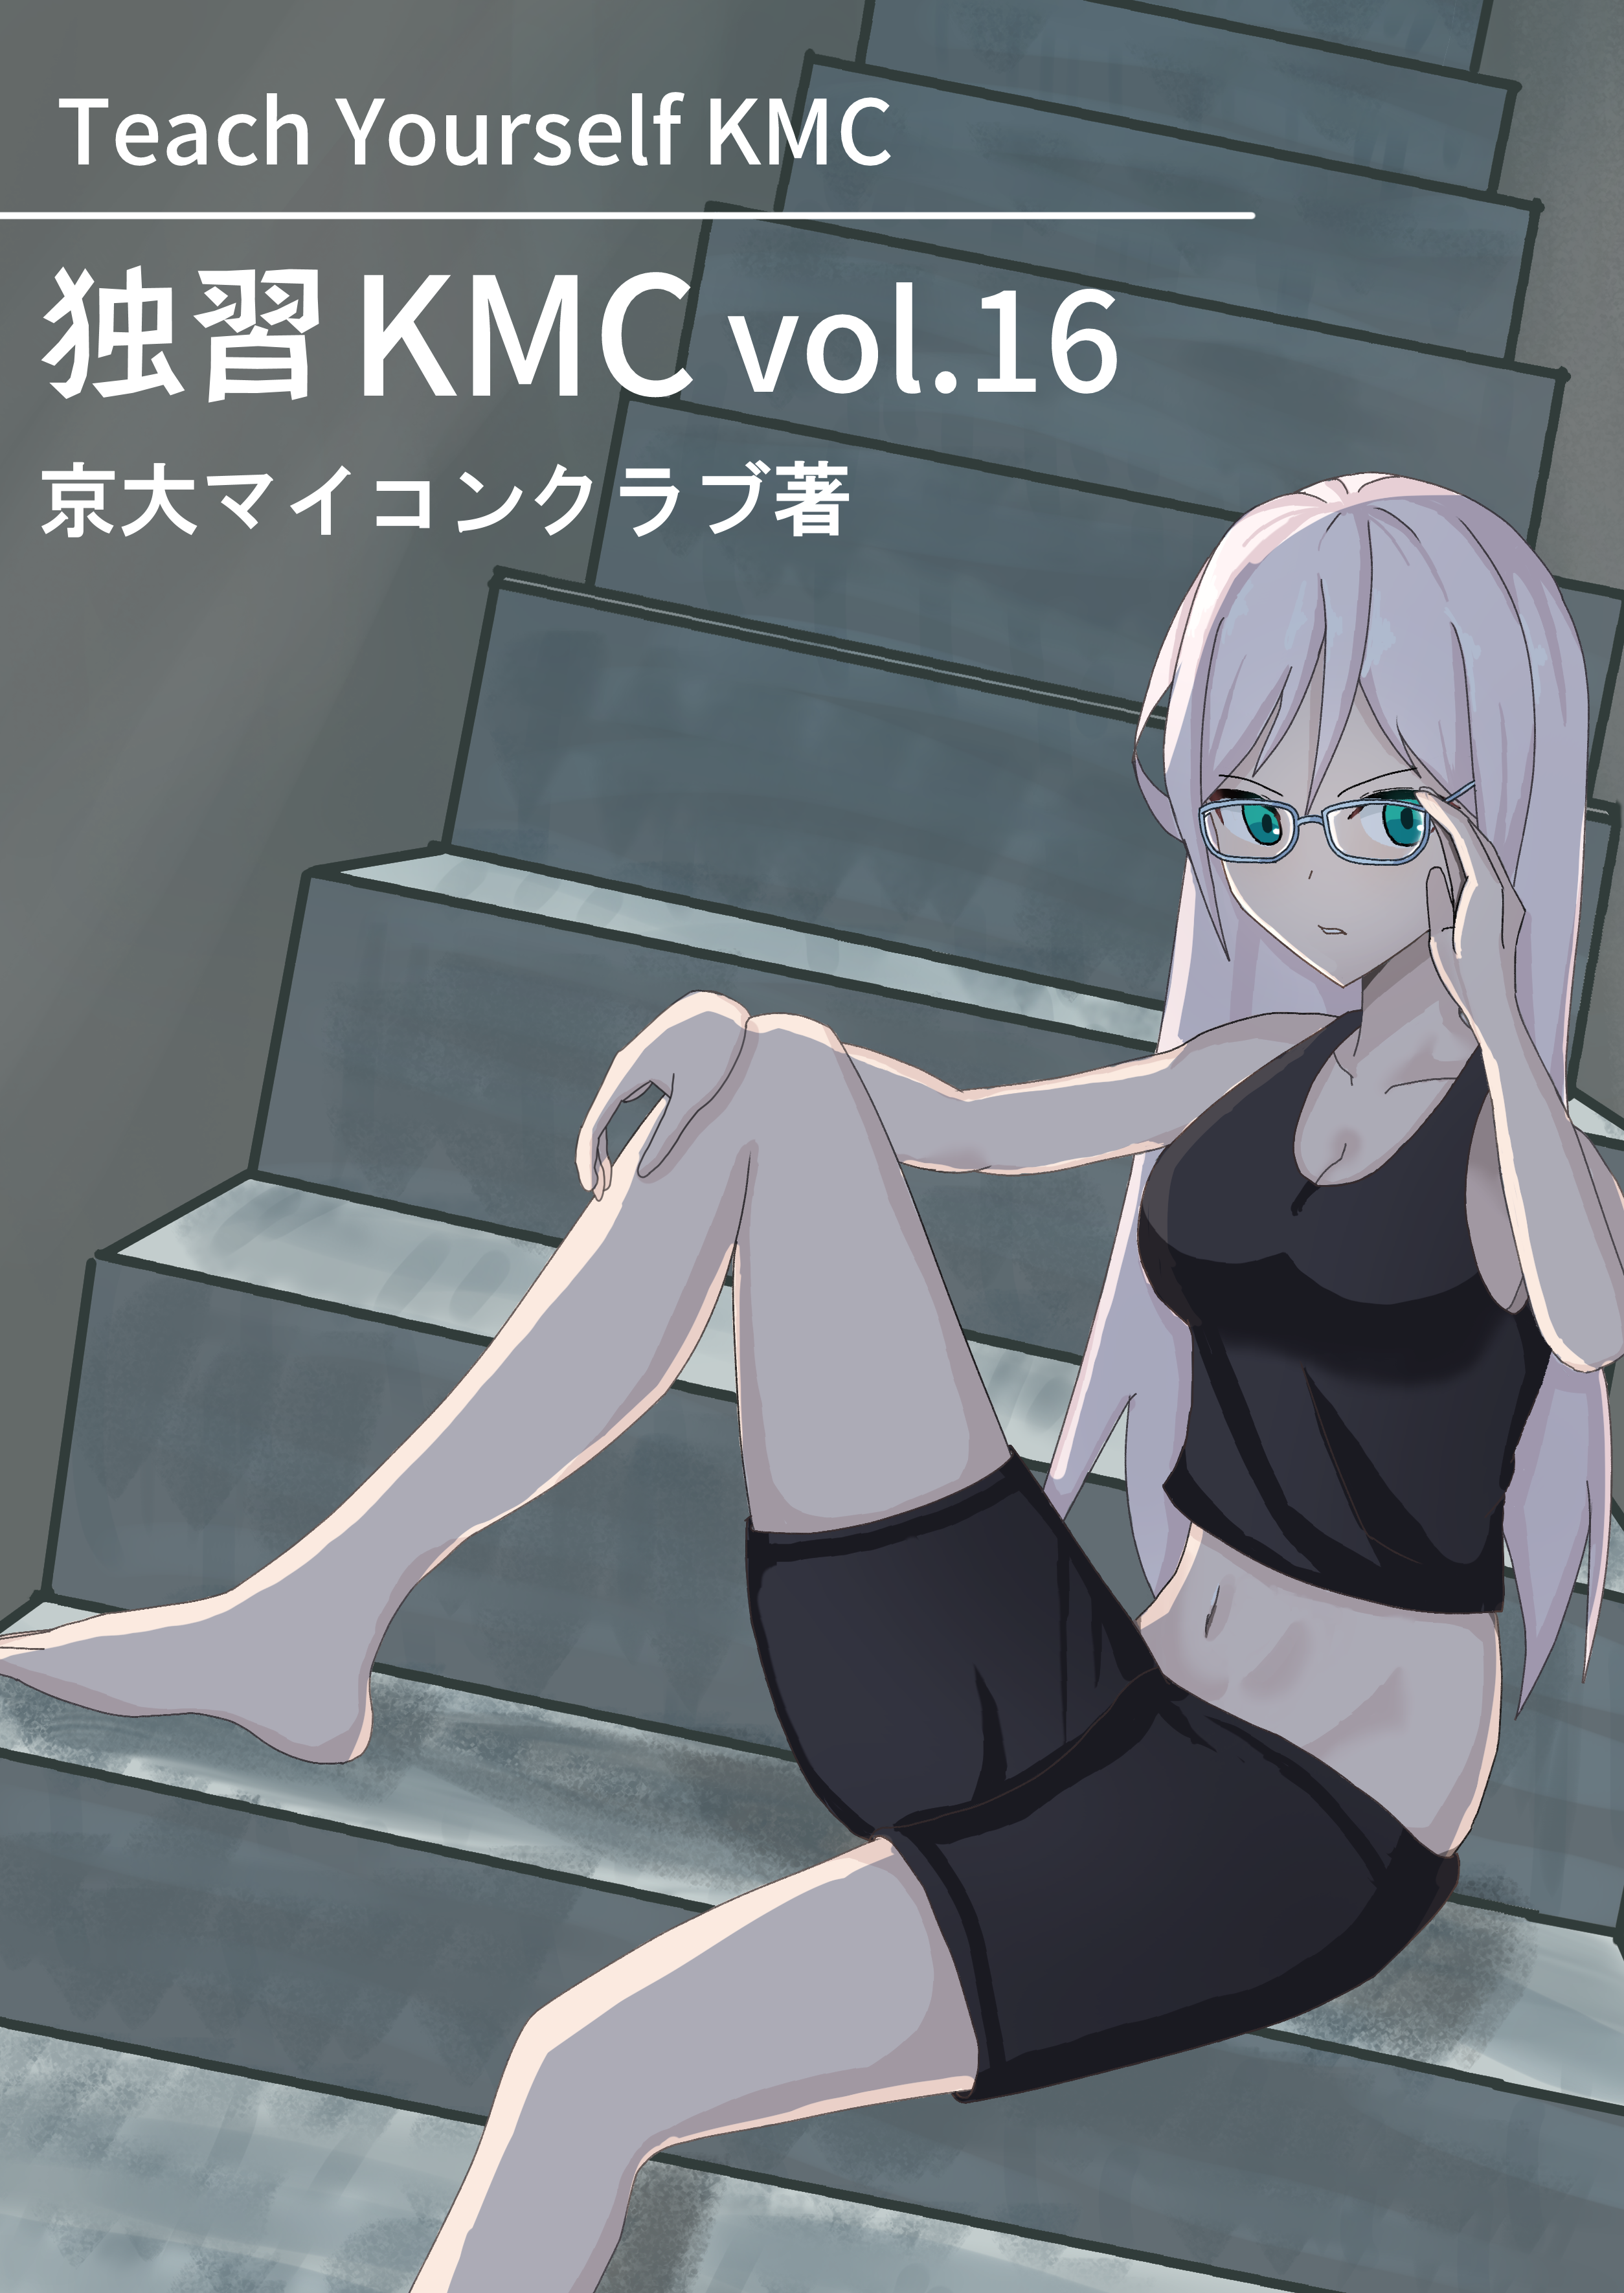
\includepdf{air2_front_5_trim.png}

\maketitle

\makeatletter
%% リンク先のURLを脚注に表示する
\let\href@orig\href
\renewcommand{\href}[2]{\href@orig{#1}{#2}\footnote{\url{#1}}}
\makeatother

% 巻頭言
\include{preface}

% 目次生成
\tableofcontents

\part{最近のKMC}
\chapter{最近のKMC --- 役職者より}
恒例の「最近のKMC」コーナーです。
最近のKMCでの活動について、様々な方から寄稿いただきました。

まずは会長と代表からです。

%\include*{recent-kmc/kaicho}
%\include*{recent-kmc/daihyo}

\chapter{最近のKMC --- 新入生プロジェクト}
次に、毎年新入生向けに開いている「新入生プロジェクト」の担当者からです。

%\include*{recent-kmc/kyopro}
%\include*{recent-kmc/minge}
%\include*{recent-kmc/oekaki}
%\include*{recent-kmc/webservice}
%\include*{recent-kmc/dtm}

\chapter{最近のKMC --- その他のプロジェクト}
KMCでは、新入生プロジェクト以外にも様々なプロジェクトが動いています。それらの担当者からもコメントをいただきました。

%\include*{recent-kmc/clocklock}
%\include*{recent-kmc/yasoba}
%\include*{recent-kmc/chalk}
%\include*{recent-kmc/heavylove}

\part{部員のコラム}
\include{test}

\include{atogaki}

%\include{kousei}

\makeatletter
%% 奥付のリンクは脚注をつけない(\hrefをオリジナルの挙動に戻す)
\let\href\href@orig
\makeatother

% 奥付ここから
\null\vfill
\section*{独習KMC vol.XX}
\hrule\vskip.5mm\hrule\vskip3mm
\begin{tabular}{ll}
20XX年XX月吉日& 初版発行\\
\end{tabular}
\vskip1em
\begin{tabular}{ll}
著作・発行& 京大マイコンクラブ\\
編集& hen=syucho\\
表紙\&裏表紙デザイン& designer's name here\\
%%挿絵& ***
\end{tabular}
\vskip1em
\begin{tabular}{ll}
メールアドレス & \href{mailto:info@kmc.gr.jp}{\nolinkurl{info@kmc.gr.jp}}\\
Web & \url{https://www.kmc.gr.jp/}\\
\end{tabular}
\vskip3mm\hrule\vskip3mm
落丁・乱丁の際は在庫がある限りお取り替えいたします。上記のメールアドレスまでご連絡ください。
% 奥付ここまで

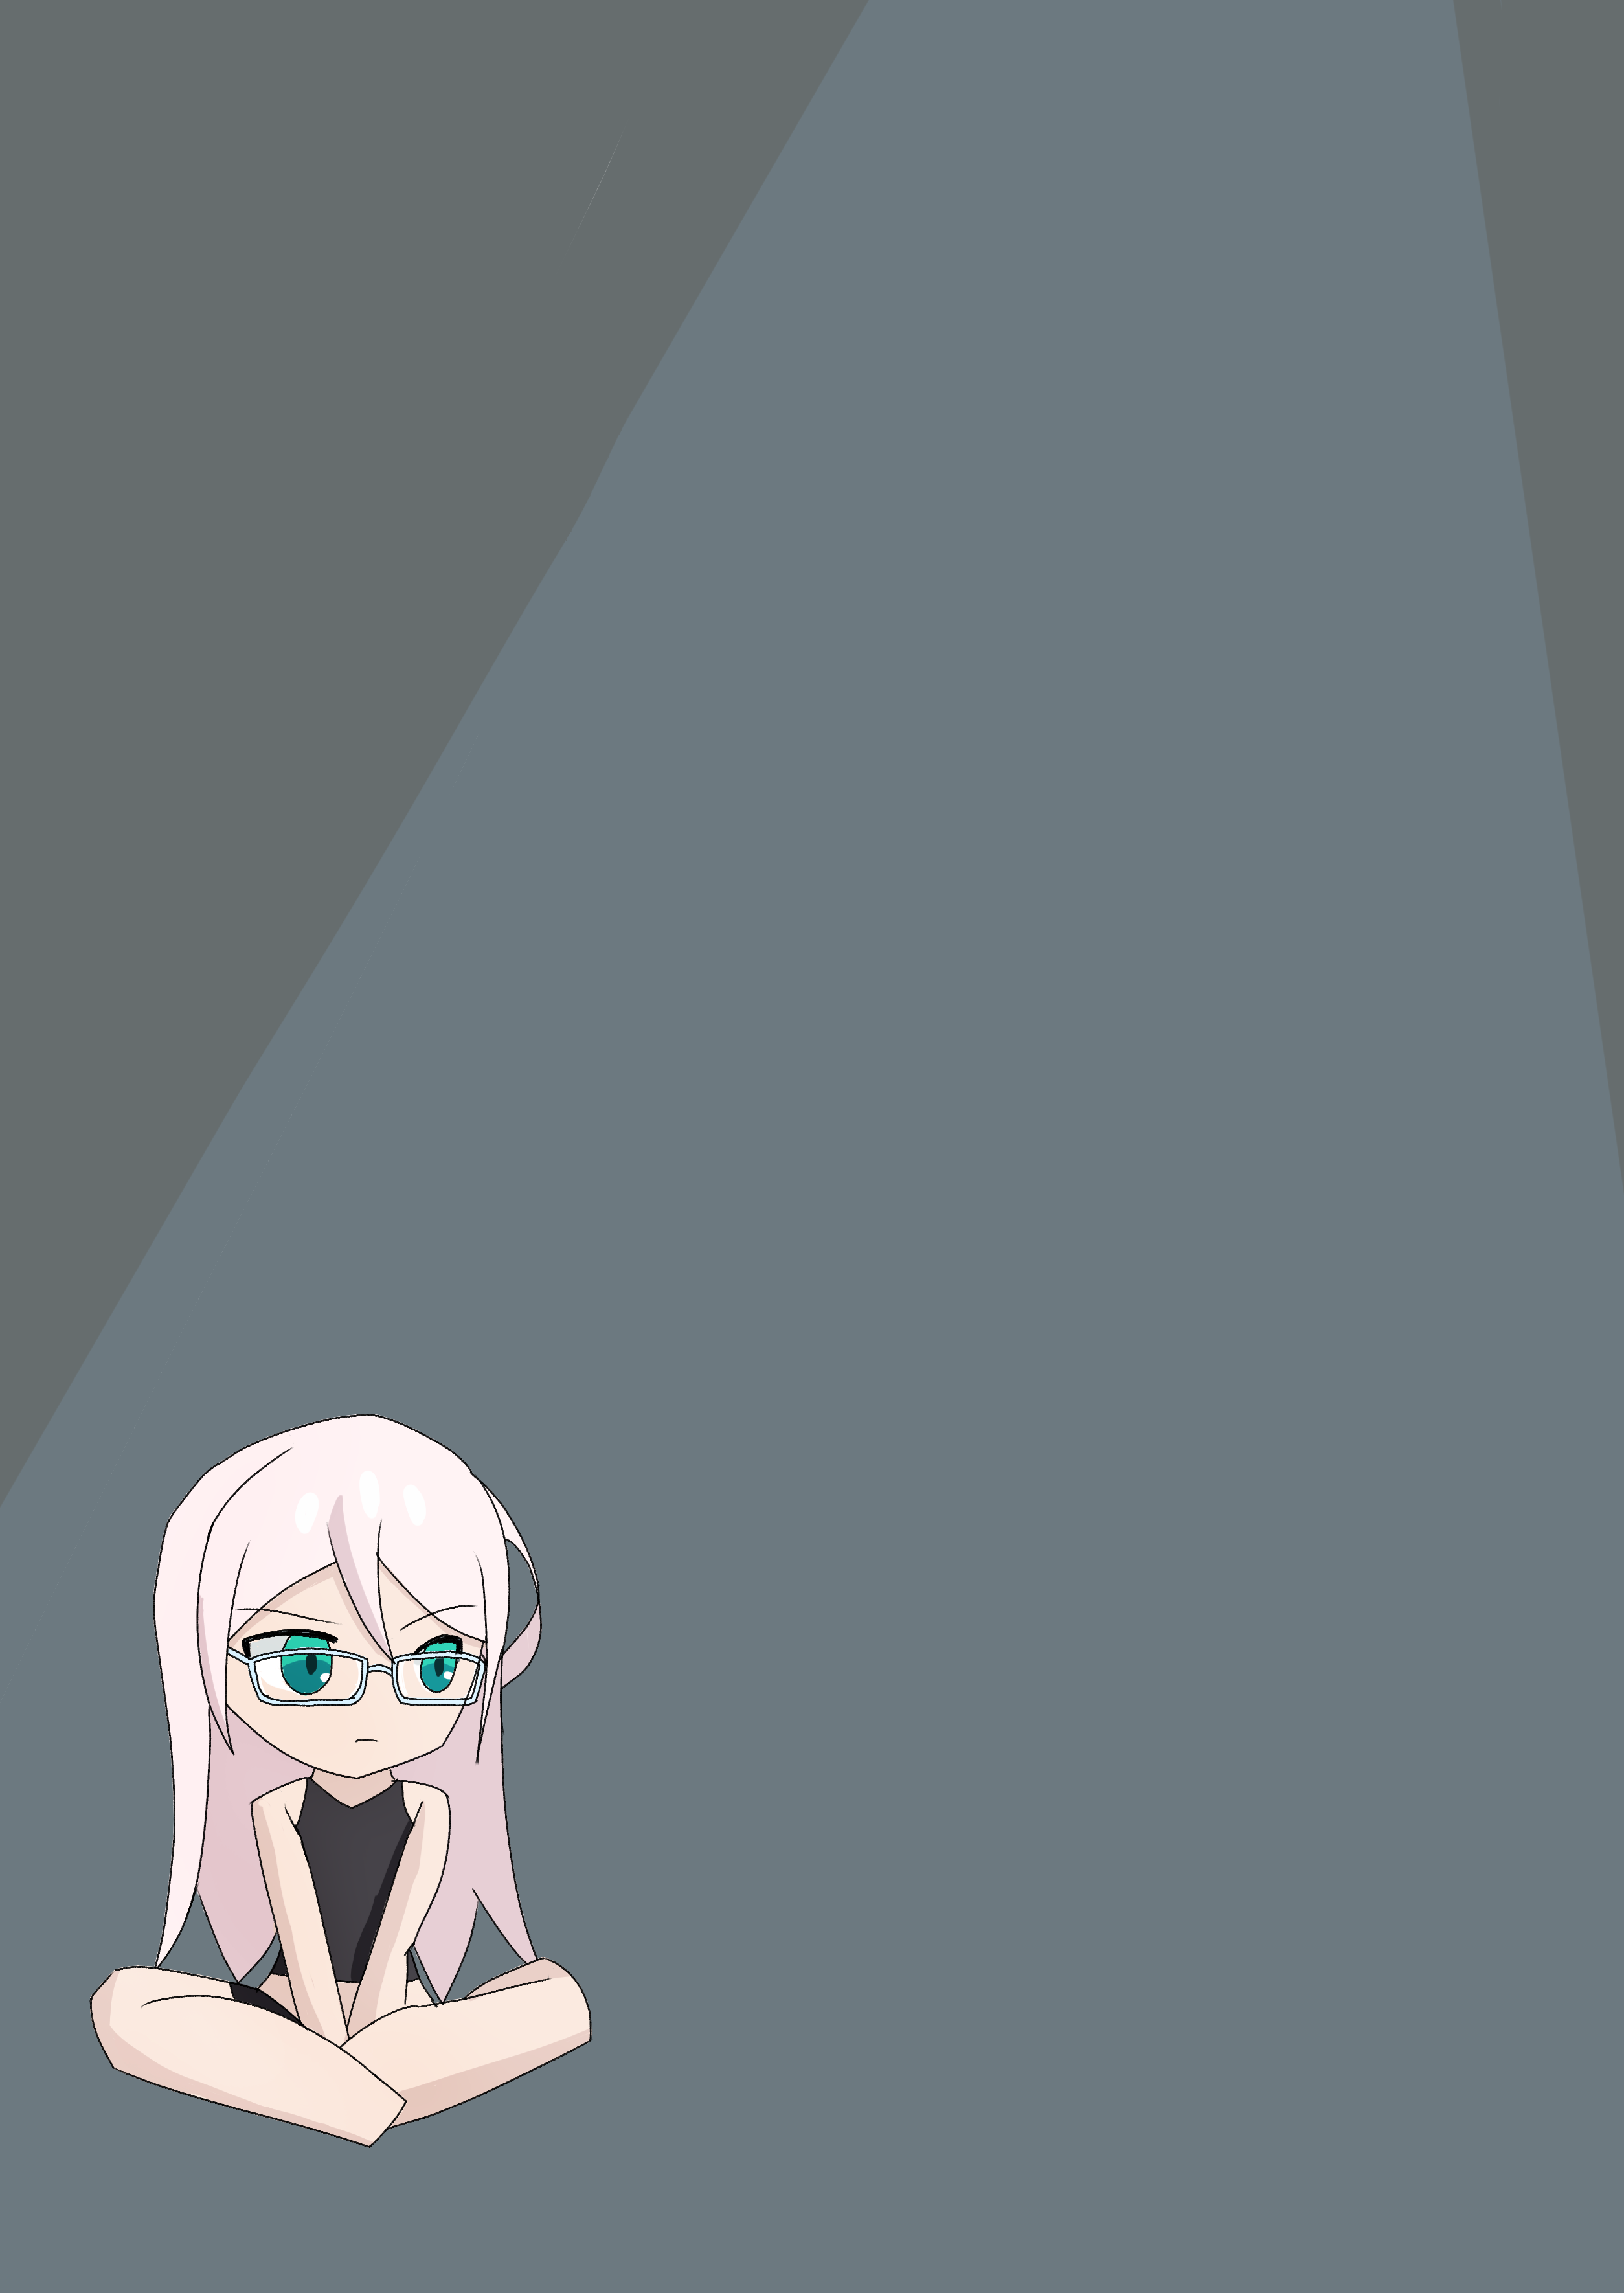
\includepdf{air2_back_trim.png}
\end{document}
